\section{Differential cross-section}

\todo{As for 90m:} 
The analysis method is very similar to the previously published ones \cite{prl111,epl101-el}. Each diagonal is analysed
separately, some steps are performed independently for each bunch. In this analysis, a different normalisation
approach is used, consequently making all $t$-independent scaling factors (e.g.~inefficiency corrections)
irrelevant.

%----------------------------------------------------------------------------------------------------
\subsection{Event reconstruction}

guide for reconstruction formulae = robustness against error sources: beam divergence, sensor pitch, misalignment, vertex term neglected, optics imperfections

One arm -- for cuts
\begin{equation}
\label{eq:kin 1a}
	\begin{aligned}
		\theta_x^* &= {v_x^{\rm N} x^{\rm F} - v_x^{\rm F} x^{\rm N}\over v_x^{\rm N} L_x^{\rm F} - v_x^{\rm F} L_x^{\rm N}}\ ,\qquad
		\theta_y^* = {1\over 2} \left( {y^{\rm N}\over L_y^{\rm N}} + {y^{\rm F}\over L_y^{\rm F}} \right)\ ,\\
		x^* &= {L_x^{\rm N} x^{\rm F} - L_x^{\rm F} x^{\rm N}\over L_x^{\rm N} v_x^{\rm F} - L_x^{\rm F} v_x^{\rm N}}\ , \\
	\end{aligned}
\end{equation}

two arm -- better resolution for already selected events
\begin{equation}
\label{eq:kin 2a}
	\begin{aligned}
		\theta_x^* &= {
				\sum v_i^2 \sum L_i x_i - \sum L_i v_i \sum v_i x_i
				\over
				\sum v_i^2 \sum L_i^2 - \sum L_i v_i \sum L_i v_i
			}\ ,\\
		\theta_y^* &= (\theta_y^{*L} + \theta_y^{*R})/2\ .\\
	\end{aligned}
\end{equation}

%------------------------------

{\bf Alignment}. The standard three-step procedure \cite{totem-ijmp} has been applied, further extended by steps improving the vertical alignment. They exploit the fact that the elastic scattering with its two anti-collinear protons can rely the alignment in the left and right arm (with an uncertainty of $20\un{\mu m}$). Furthermore, the horizontal RPs in right arm showed a hit distribution usable for vertical alignment in addition to the other technique based on the vertical RPs. Together, the two methods reduce the uncertainty to about $70\un{\mu m}$. The horizontal alignment and rotation about the beam have been determined with the standard approach, with uncertainties $30\un{\mu m}$ and $2\un{m rad}$, respectively. Propagating the uncertainties to the reconstructed angles, Eq.~(\ref{eq:kin 2a}), gives $0.28\un{\mu rad}$ ($0.19\un{\mu rad}$) for horizontal (vertical) angle. The error of the RP rotations would cause admixture of $\theta_y^*$ to $\theta_x^*$ with proportionality constant having standard deviation $0.005$.

% the observed hit inefficiencies -- possible asymmetries -- discuss ???
% mention final alignment check = 2D Gaussian fit of $\theta_x^*$ vs.~$\theta_y^*$ from both diagonals ??

%------------------------------

{\bf Optics}. The optics matching method \cite{totem-optics} has been applied. The residual uncertainty has a form of factors scaling the reconstructed scattering angles:
% double-arm; 
$0.34\un{\%}$ (horizontal) and $0.25\un{\%}$ (vertical), including the effects of magnet harmonics.


%------------------------------

{\bf Resolution}. Good knowledge of statistical fluctuations in the event reconstruction is essential for several steps in differential cross-section reconstruction. The fluctuations in $\theta_y^*$ are mostly due to the beam divergence phenomenon and can be studied by comparing the angles reconstructed from the left and right arm. If the divergences of both beams are the same (verified by emittance measurements with uncertainty of $25\un{\%}$), then the beam divergence distribution can be de-convoluted from the distribution of the left-right differences. The beam divergence has shown very small deviations from Gaussian shape (taken as a source of uncertainty) but increasing width with time. Thus the $\theta_y^*$ (Eq.~(\ref{eq:kin 2a})) resolution degraded from initial $4.3$ to $4.8\un{\mu rad}$ at the end of the fill. In the horizontal projection, a different method must be used since the one-arm reconstruction, Eq.~(\ref{eq:kin 1a}), is strongly influenced by sensor resolution. First, the beam divergence is calculated from the vertex $x^*$ spread by dividing by the known $\beta^*$: it grew from $0.75$ to $0.9\un{\mu rad}$ during the fill. Second, the beam-divergence component is subtracted from the standard deviation of the right-left difference in $\theta_x^*$, yielding (time-independent) contribution from the sensor resolution: $10.7\un{\mu m}$ (45 top -- 56 bottom) and $12.1\un{\mu m}$ (45 bottom -- 56 top). This can be propagated to the two-arm resolution in $\theta_x^*$, Eq.~({\ref{eq:kin 2a}}), which is almost purely determined by the beam divergence: it rose from $0.54$ to $0.65\un{\mu rad}$ during the fill. 


%----------------------------------------------------------------------------------------------------
\subsection{Differential cross-section}

\todo{As for 90m:} 
For a given $t$ bin, the value of differential cross-section is evaluated by selecting and counting elastic events as follows
\begin{equation}
{\d\sigma\over \d t}(\hbox{bin}) =
	{\cal N}\, {\cal U}({\rm bin})\, {\cal B}\ 
	{\sum\limits_{t \in \hbox{bin}} {\cal A}(\theta_x^*, \theta_y^*)\, {\cal E}(\theta_y^*)\over \Delta t}\ ,
\end{equation}
where $\Delta t$ is the width of the bin, ${\cal N}$ is a normalisation factor and the other symbols stand for various correction factors:
 ${\cal U}$ for unfolding, ${\cal B}$ for background subtraction, ${\cal A}$ for acceptance correction and ${\cal E}$ for detection and reconstruction efficiency.


{\bf Tagging}. The cuts used to select the elastic events are summarized in Tab.~\ref{tab:cuts}, all are applied at $4\sigma$-level. Cuts 1 and 2 require the reconstructed-track collinearity between the left and right arm. Cut 3 ensures that the protons come from the same vertex (horizontally). Thanks to the very good resolution, the collinearity cuts are very strong and consequently the other possible cuts (cf.~\cite{epl101-el}) bring no significant improvement. The tagging efficiency is studied by applying the cuts also at $5\un{\sigma}$-level. This selection yields $0.3\un{\%}$ more events, almost uniformly in $|t|$ (at very low $|t|$ in increases to $\approx 1\un{\%}$ -- anyway well in systematics). This kind of inefficiency is irrelevant for this analysis.

\begin{table}
\caption{The elastic selection cuts. The superscripts R and L refer to the right and left arm. The $\alpha \theta_x^*$ term in cut 3 is intended to absorb possible effects of residual optics imperfections. The right-most column gives a typical RMS of the cut distribution.
}
\label{tab:cuts}
\begin{center}
\vskip-3mm
\begin{tabular}{ccc}\hline\hline
number & cut & RMS ($\equiv 1\sigma$)\cr\hline
1 & $\theta_x^{*\rm R} - \theta_x^{*\rm L}$				& $3.9\un{\mu rad}$	\cr
2 & $\theta_y^{*\rm R} - \theta_y^{*\rm L}$				& $1.0\un{\mu rad}$	\cr
3 & $x^{*\rm R} - x^{*\rm L} - \alpha \theta_x^*$		& $250\un{\mu m}$ 	\cr\hline\hline
\end{tabular}
\end{center}
\end{table}


%-------------------------
{\bf Background}.
% background = impurity of the cuts above
Method: plot a cut quantity ($\Delta \theta_{x,y}^*$) under various cut combinations. Separation of signal and background: central peak (signal) stays, while tails (background) drop. Residual after all cuts $\rightarrow$ interpolate to signal region $\rightarrow$ background negligible ($B /(B+S) < 0.1\un{\%}$, for both x and y cuts). Further test: $|t|$-distributions with one cut released -- additional events (background, $\approx 0.3\un{\%}$) distributed almost uniformly over $|t|$ (no peaking), except in very low $|t|$ -- small increase to $\approx 1.5\un{\%}$ (anyway, well in within systematics).


%-------------------------

{\bf Acceptance correction}. Beyond the usual acceptance limitations -- sensor edge (relevant for low $|\theta^*_y|$) and LHC apertures (high $|\theta_y^*|$) -- two additional ones have been identified. Both stem from the horizontal RPs interfering with the elastic protons, resulting in uncertain detection efficiency. Consequently, an additional acceptance restriction $-50 < \theta_x^* < 80\un{\mu rad}$ has been adopted to avoid the interference regions. Otherwise, the standard correction technique \cite{8tev-90m} has been applied, comprising a geometrical correction (exploiting the verified azimuthal symmetry) and a correction for smearing around the acceptance limits.


%-------------------------

{\bf Efficiency corrections} include corrections for inefficiencies from various sources: trigger inefficiency ${\cal I}_{\rm trig}$, reconstruction inefficiency ${\cal I}_{\rm det}$ and pile-up inefficiency ${\cal I}_{\rm PU}$ (RPs unable to resolve multiple tracks):

\begin{equation}
\label{efficiency}
	\begin{aligned}
		{\cal E}(\theta_y^*) &= {1\over 1 - {\cal I}_{\rm trig}} {1\over 1 - {\cal I}_{\rm det}(\theta_y^*)} {1\over 1 - {\cal I}_{\rm PU}}\ ,\\
		{\cal I}_{\rm det}(\theta_y^*) &= \sum\limits_{i\in \rm RPs} {\cal I}^i_{3/4}(\theta_y^*) + 2 {\cal I}_{2/4}\\
	\end{aligned}
\end{equation}

\> ``standard procedure'' for the standard contributions (ref. to previous publications?): ``3-out-of-4'' (uncorrelated 1-RP inefficiencies), ``shower in near'' (near-far correlated) and ``pile-up'' (coincidence with beam-halo or any other particle)

\> 3-out-of-4 results
\>> right arm: typical results (near $\approx 98\un{\%}$, far $\approx 96.5\un{\%}$ efficiency)
\>> left arm: efficiency in far RP unexpectedly low ($\approx 90\un{\%}$) -- due to showers in horizontal RPs (horizontal in left arm closer that in the right one) -- but experimentally determinable and thus fully correctable

\> pile-up results shown in Fig.~\ref{fig:overview}
\>> strong time-dependece: linear rise within the data-taking periods, decrease in beam cleanings


%-------------------------

{\bf Unsmearing} The standard per-bin technique has been applied \cite{8tev-90m}. Due to the very small beam divergence, the effect is negligible for all bins except the very low-$|t|$ ones where the rapid cross-section growth appears because of the Coulomb interaction (correction $< 2.5\un{\%}$). For the uncertainty estimate, the uncertainties of $\theta_x^*$ and $\theta_y^*$ resolutions (to accommodate the full time variation) as well as fit-model dependence have been considered, each contribution giving few per-mille for the lowest-$|t|$ point.

\iffalse
\> but time-dependent smearing sigma, determined from the variation of $\theta_y^{*R} - \theta_y^{*L}$
\>> mention the subtlety with $\sigma(\theta_x^*)$ ?? Cannot be measured directly. The only handle comes from the emittances (crude only). But (at least for low-$|t|$), the impact of $\theta_x^*$ smearing is small -- the value of $\theta^*$ is mostly made by $\theta_y^*$, therefore $\theta_x^*$ must be very small. Consequently, $\Delta t_x = 2 \theta_x^* \Delta \theta_x^* \approx 0$
\fi

%-------------------------
{\bf Normalisation}. Same integral between $|t| = 0.014$ and $0.2030\un{GeV^2}$ as DS1 from \cite{prl111}, where luminosity-independent calibration was applied. Leading uncertainty: $4.2\un{\%}$ from luminosity-independent method, transfer negligible ($0.5\un{\%}$).
% stat: 0.3%, syst: 0.3% (DS2 at 90m), 0.3% (1km)


%-------------------------

The {\bf binning} has been optimised with respect to two aspects. At low $|t|$, the bin size has been set to the triple of the resolution in $t$. At higher $|t|$, a fixed statistical fluctuation of $4\un{\%}$ has been targeted.

%-------------------------
{\bf Systematic uncertainties}

\> ``standard procedure'' (ref. to previous publications?) of uncertainty assessment

\> leading uncertainties: residual misalignment (very low-$|t|$), normalisation (flat)

\> compatible results obtained if data right after or right before beam cleaning are used



%----------------------------------------------------------------------------------------------------
\subsection{Final data merging}

\> merging datasets + diagonals

\> central values

\> statistical uncertainties

\> systematic uncertainties


\input data_table.tex


\begin{figure*}
\vskip-5mm
\begin{center}
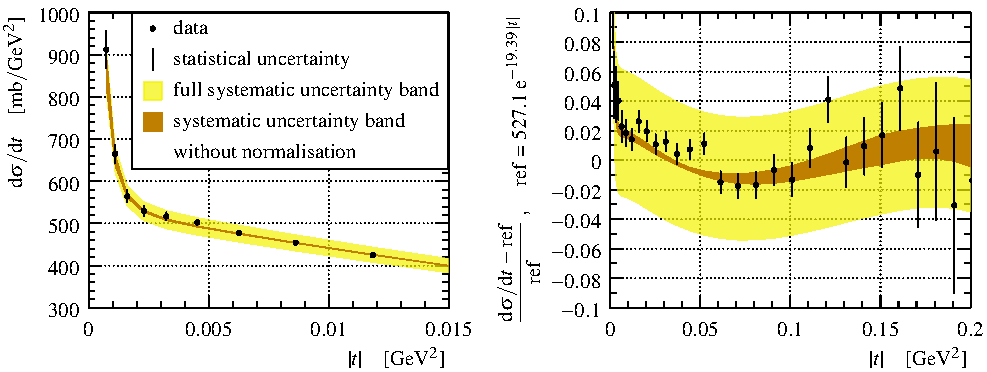
\includegraphics[width=18cm]{fig/t_dist_tabulation.pdf}
\vskip-3mm
\caption{Differential cross-section. \todo{shall we keep all 3?} \todo{describe!}}
\label{fig:dsdt}
\end{center}
\end{figure*}

\> present/comment Fig.~\ref{fig:dsdt}


